\documentclass[12pt, oneside]{article}

\usepackage[letterpaper, scale=0.89, centering]{geometry}
\usepackage{fancyhdr}
\setlength{\parindent}{0em}
\setlength{\parskip}{1em}

\pagestyle{fancy}
\fancyhf{}
\renewcommand{\headrulewidth}{0pt}
\rfoot{\href{https://creativecommons.org/licenses/by-nc-sa/2.0/}{CC BY-NC-SA 2.0} Version \today~(\thepage)}

\usepackage{amssymb,amsmath,pifont,amsfonts,comment,enumerate,enumitem}
\usepackage{currfile,xstring,hyperref,tabularx,graphicx,wasysym}
\usepackage[labelformat=empty]{caption}
\usepackage{xcolor}
\usepackage{multicol,multirow,array,listings,tabularx,lastpage,textcomp,booktabs}

\lstnewenvironment{algorithm}[1][] {   
    \lstset{ mathescape=true,
        frame=tB,
        numbers=left, 
        numberstyle=\tiny,
        basicstyle=\rmfamily\scriptsize, 
        keywordstyle=\color{black}\bfseries,
        keywords={,procedure, div, for, to, input, output, return, datatype, function, in, if, else, foreach, while, begin, end, }
        numbers=left,
        xleftmargin=.04\textwidth,
        #1
    }
}
{}

\newcommand\abs[1]{\lvert~#1~\rvert}
\newcommand{\st}{\mid}

\newcommand{\cmark}{\ding{51}}
\newcommand{\xmark}{\ding{55}}
 
\begin{document}
\begin{flushright}
    \StrBefore{\currfilename}{.}
\end{flushright} \section*{Week4 wednesday}


Regular sets are not the end of the story
\begin{itemize}
    \item Many nice / simple / important sets are not regular
    \item Limitation of the finite-state automaton model: Can't ``count", Can only remember finitely far into the past,
    Can't backtrack, Must make decisions in ``real-time"
    \item We know actual computers are more powerful than this model...
\end{itemize}

The {\bf next} model of computation. Idea: allow some memory of unbounded size. How? 
\begin{itemize}
    \item To generalize regular expressions: {\bf context-free grammars}\\
    \item To generalize NFA: {\bf Pushdown automata}, which is like an NFA with access to a stack: 
    Number of states is fixed, number of entries in stack is unbounded. At each step
    (1) Transition to new state based on current state, letter read, and top letter of stack, then
    (2) (Possibly) push or pop a letter to (or from) top of stack. Accept a string iff
    there is some sequence of states and some sequence of stack contents 
    which helps the PDA processes the entire input string and ends in an accepting state.
\end{itemize}

\vfill

\vfill

Is there a PDA that recognizes the nonregular language $\{0^n1^n \mid n \geq 0 \}$?

\vfill

\newpage


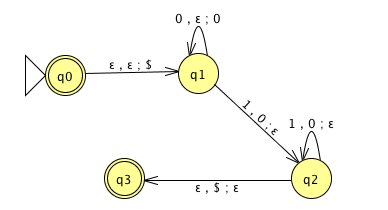
\includegraphics[width=4in]{../../resources/machines/Lect9PDA.png}

The PDA with state diagram above can be informally described as:
\begin{quote}
    Read symbols from the input. As each 0 is read, push it onto the stack. 
    As soon as 1s are seen, pop a 0 off the stack for each 1 read. 
    If the stack becomes empty and we are at the end of the input string, accept the input. 
    If the stack becomes empty and there are 1s left to read, 
    or if 1s are finished while the stack still contains 0s, or if any 0s
    appear in the string following 1s, 
    reject the input.
\end{quote}
    

Trace the computation of this PDA on the input string $01$.

\vfill
    
Trace the computation of this PDA on the input string $011$.

\vfill


A PDA recognizing the set $\{ \hspace{1.5 in} \}$ can be informally described as:
\begin{quote}
    Read symbols from the input. As each 0 is read, push it onto the stack. 
    As soon as 1s are seen, pop a 0 off the stack for each 1 read. 
    If the stack becomes empty and there is exactly one 1 left to read, read that 1 and accept the input. 
    If the stack becomes empty and there are either zero or more than one 1s left to read, 
    or if the 1s are finished while the stack still contains 0s, or if any 0s appear in the input following 1s, 
    reject the input.
\end{quote}
Modify the state diagram below to get a PDA that implements this description:

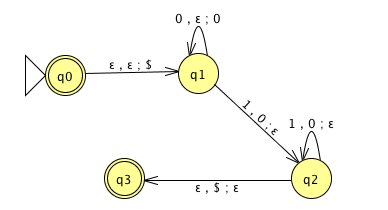
\includegraphics[width=4in]{../../resources/machines/Lect9PDA.png}


\newpage
{\bf Definition} A {\bf pushdown automaton} (PDA) is  specified by a  $6$-tuple $(Q, \Sigma, \Gamma, \delta, q_0, F)$
where $Q$ is the finite set of states, $\Sigma$ is the input alphabet,  $\Gamma$ is the stack alphabet,
\[
    \delta: Q \times \Sigma_\varepsilon  \times  \Gamma_\varepsilon \to \mathcal{P}( Q \times \Gamma_\varepsilon)
\]
is the transition function,  $q_0 \in Q$ is the start state, $F \subseteq  Q$ is the set of accept states.
    

\vspace{90pt}
Draw the state diagram and give the formal definition of a PDA with $\Sigma = \Gamma$.

\vfill

Draw the state diagram and give the formal definition of a PDA with $\Sigma \cap \Gamma = \emptyset$.
    
\vfill

    
\newpage
{\it Extra practice}: Consider the state diagram of a PDA with input alphabet 
$\Sigma$ and stack alphabet $\Gamma$.

\begin{center}
\begin{tabular}{|c|c|}
\hline
Label & means \\
\hline
$a, b ; c$ when $a \in \Sigma$, $b\in \Gamma$, $c \in \Gamma$ 
& \hspace{3in} \\
& \\
& \\
& \\
& \\
&\\
\hline
$a, \varepsilon ; c$ when $a \in \Sigma$, $c \in \Gamma$ 
& \hspace{3in} \\
& \\
& \\
& \\
& \\
&\\
\hline
$a, b ; \varepsilon$ when $a \in \Sigma$, $b\in \Gamma$
& \hspace{3in} \\
& \\
& \\
& \\
& \\
&\\
\hline
$a, \varepsilon ; \varepsilon$ when $a \in \Sigma$
& \hspace{3in} \\
& \\
& \\
& \\
& \\
&\\
\hline
\end{tabular}
\end{center}


How does the meaning change if $a$ is replaced by $\varepsilon$?

{\it Note: alternate notation is to replace $;$ with $\to$}
 \vfill
\section*{Week4 friday}


    
For the PDA state diagrams below, $\Sigma = \{0,1\}$.


\begin{center}
\begin{tabular}{c c}
Mathematical description of language & State diagram of PDA recognizing language\\
\hline
& $\Gamma = \{ \$, \#\}$ \hspace{2.3in} \\
& \\
& 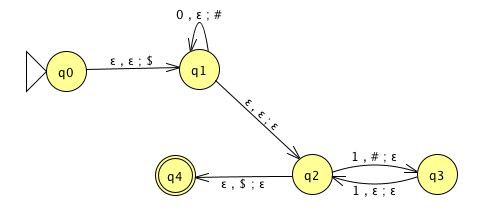
\includegraphics[width=3.5in]{../../resources/machines/Lect10PDA1.png}\\
& \\
& \\
\hline
& $\Gamma = \{ {@}, 1\}$ \hspace{2.3in} \\
& \\
& 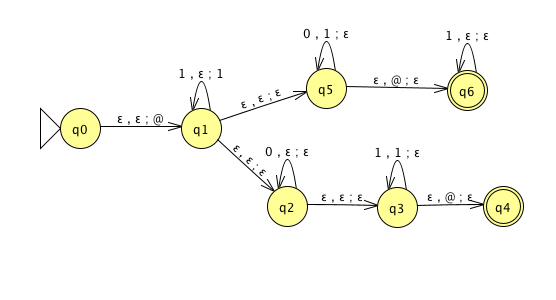
\includegraphics[width=3.5in]{../../resources/machines/Lect10PDA2.png}\\
& \\
& \\
\hline
& \\
& \\
& \\
$\{ 0^i 1^j 0^k \mid i,j,k \geq 0 \}$ & \\
& \\
& \\
\end{tabular}
\end{center}

\newpage
{\it Big picture}: PDAs were motivated by wanting to add some memory of unbounded size to NFA. How 
do we accomplish a similar enhancement of regular expressions to get a syntactic model that is 
more expressive?

DFA, NFA, PDA: Machines process one input string at a time; the computation of a machine on its input string 
reads the input from left to right.

Regular expressions: Syntactic descriptions of all strings that match a particular pattern; the language 
described by a regular expression is built up recursively according to the expression's syntax

{\bf Context-free grammars}: Rules to produce one string at a time, adding characters from the middle, beginning, 
or end of the final string as the derivation proceeds.


\begin{center}
  \hspace{-0.25in}\begin{tabular}{|p{2in}cp{4in}|}
  \hline 
  Term & Typical symbol & Definition \\
  \hline\hline
  {\bf Context-free grammar} (CFG) & $G$ & $G = (V, \Sigma, R, S)$ \\
  {\bf Variables}& $V$ & Finite  set of symbols that represent phases in production pattern\\
  {\bf Terminals} & $\Sigma$ & Alphabet of symbols of strings generated  by CFG \\
  & & $V \cap \Sigma = \emptyset$ \\
  {\bf Rules}& $R$ & Each rule is  $A \to u$ with $A \in V$ and $u  \in (V  \cup \Sigma)^*$\\
  Start variable&  $S$  & Usually  on LHS of first / topmost rule \\
  {\bf Derivation} & & Sequence  of substitutions in a  CFG \\
  & $S \implies \cdots \implies w$ & Start with start variable, apply one rule to one occurrence of a variable at a time\\
  {\bf Language} generated by the CFG $G$ & $L(G)$ &$\{  w \in \Sigma^* \mid \text{there is  derivation in $G$ that ends
  in $w$} \} = \{  w \in \Sigma^* \mid S \implies^* w \}$\\
  {\bf Context-free language} & & A language that is the language generated by some CFG\\
  \hline
  Sipser pages 102-103 & &\\
  \hline
  \end{tabular}
  \end{center}
  
{\bf Examples of context-free grammars, derivations in those grammars, and the languages generated by those grammars}
  
$G_1 =  (\{S\}, \{0\}, R, S)$ with rules
  \begin{align*}
    &S \to 0S\\
    &S \to 0\\
  \end{align*}
  In  $L(G_1)$ \ldots 
  
  \vspace{110pt}
  
  Not in $L(G_1)$ \ldots 

  \vspace{110pt}

\newpage
  $G_2 =  (\{S\}, \{0,1\}, R, S)$
  \[
  S \to 0S \mid 1S \mid \varepsilon
  \]
  In  $L(G_2)$ \ldots 
  
  \vspace{110pt}
  
  Not in $L(G_2)$ \ldots 

  \vspace{110pt}

  $(\{S, T\}, \{0, 1\}, R, S)$ with  rules
  \begin{align*}
  &S \to T1T1T1T \\
  &T \to  0T \mid 1T \mid \varepsilon
  \end{align*}

  In  $L(G_3)$ \ldots 
  
  \vspace{110pt}
  
  Not in $L(G_3)$ \ldots 

  \vspace{110pt}

\newpage
  $G_4 =  (\{A, B\}, \{0, 1\}, R, A)$ with rules
  \[
    A \to 0A0 \mid  0A1 \mid 1A0  \mid 1A1 \mid  1
  \]
  In  $L(G_4)$ \ldots 
  
  \vspace{110pt}
  
  Not in $L(G_4)$ \ldots 

  \vspace{110pt}

  
{\it Extra practice}: Is there a CFG $G$ with $L(G) = \emptyset$?
 \vfill
\section*{Week6 friday}


{\bf Nondeterministic Turing machine}

At any point in the computation, the nondeterministic machine may proceed according to 
several possibilities: $(Q, \Sigma, \Gamma, \delta, q_0, q_{acc}, q_{rej})$ where 
\[
\delta: Q \times \Gamma \to \mathcal{P}(Q \times \Gamma \times \{L, R\})  
\]
The computation of a nondeterministic Turing machine is a tree with branching
when the next step of the computation has multiple possibilities. A nondeterministic
Turing machine accepts a string exactly when some branch of the computation tree 
enters the accept state.

Given a nondeterministic machine, we can use a $3$-tape Turing machine to 
simulate it by doing a breadth-first search of computation tree: one tape 
is ``read-only'' input tape, one tape simulates the tape of the nondeterministic
computation, and one tape tracks nondeterministic branching. {\tiny Sipser page 178} 

\vfill
Two models of computation are called {\bf equally expressive} when 
every language recognizable with the first model is recognizable with the second, and vice versa.

{\bf  Church-Turing Thesis} (Sipser p. 183): The informal notion of algorithm is formalized completely  and correctly by the 
formal definition of a  Turing machine. In other words: all reasonably expressive models of 
computation are equally expressive with the standard Turing machine.

\vfill

\newpage


A language $L$ is {\bf recognized by} a Turing machine $M$ means

\vspace{15pt}

A Turing  machine  $M$ {\bf  recognizes} a language $L$ if means

\vspace{15pt}

A Turing machine $M$ is a {\bf decider}  means

\vspace{15pt}

A language  $L$ is {\bf decided by} a Turing  machine  $M$  means

\vspace{15pt}

A  Turing machine $M$ {\bf decides} a language $L$ means

\vspace{15pt}

Fix $\Sigma = \{0,1\}$, $\Gamma = \{ 0, 1, \textvisiblespace\}$ for the Turing machines with  the following state diagrams:
  
  \begin{center}
  \begin{tabular}{|c|c|}
  \hline
  \hspace{0.8in}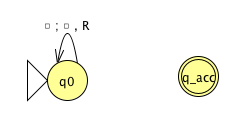
\includegraphics[width=2in]{../../resources/machines/Lect14TM1.png} \phantom{\hspace{0.8in}}&\hspace{0.8in} 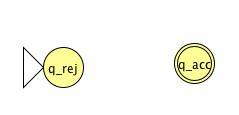
\includegraphics[width=2in]{../../resources/machines/Lect14TM2.png} \phantom{\hspace{0.8in}}\\
  Decider? Yes~~~/ ~~~No
  &Decider? Yes~~~/ ~~~No\\
  & \\
  \hline
  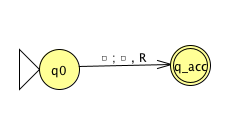
\includegraphics[width=2in]{../../resources/machines/Lect14TM3.png} & 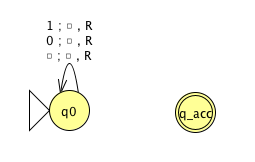
\includegraphics[width=2in]{../../resources/machines/Lect14TM4.png} \\
  Decider? Yes~~~/ ~~~No
  &Decider? Yes~~~/ ~~~No\\
  & \\
  
  \hline
  \end{tabular}
  \end{center}
  \newpage



{\bf Claim}: If two languages  (over a fixed alphabet  $\Sigma$) are Turing-recognizable, then  their union  is  as well.

{\bf Proof using Turing machines}:

\vfill

{\bf Proof using nondeterministic Turing machines}: 

\vfill  

{\bf  Proof using enumerators}:

\vfill

\newpage
    
{\bf Describing  Turing machines} (Sipser p. 185)


To define a Turing machine, we could give a 
\begin{itemize}
\item {\bf Formal definition}: the $7$-tuple of parameters including set of states, 
input alphabet, tape alphabet, transition function, start state, accept state, and reject state; or,
\item {\bf Implementation-level definition}: English prose that describes the Turing machine head 
movements relative to contents of tape, and conditions for accepting / rejecting based on those contents.
\item {\bf High-level description}: description of algorithm (precise sequence of instructions), 
without implementation details of machine. As part of this description, can ``call" and run 
another TM as a subroutine.
\end{itemize}


The Church-Turing thesis posits that each algorithm can be implemented by some Turing machine

High-level descriptions of  Turing machine algorithms are written as indented text within quotation marks.   

Stages of the algorithm are typically numbered consecutively.

The first line specifies the input to the machine, which must be a string.
This string may be the encoding of some object or  list of  objects.  

{\bf Notation:} $\langle O \rangle$ is the string that encodes the object $O$.
$\langle O_1, \ldots, O_n \rangle$ is the string that encodes the list of objects $O_1, \ldots, O_n$.

{\bf Assumption}: There are Turing  machines that can be called as subroutines
to decode the string representations of common objects and  interact with these objects as intended
(data structures).
  
For example, since there are algorithms to answer each of the following questions,
by Church-Turing thesis, there is a Turing machine that accepts exactly those strings for which the 
answer to the question is ``yes''
\begin{itemize}
    \item Does a string over $\{0,1\}$ have even length?

    \vfill

    \item Does a string over $\{0,1\}$ encode a string of ASCII characters?\footnote{An introduction to ASCII 
    is available on the w3 tutorial \href{https://www.w3schools.com/charsets/ref_html_ascii.asp}{here}.}

    \vfill

    \item Does a DFA have a specific number of states?

    \vfill

    \item Do two NFAs have any state names in common?

    \vfill

    \item Do two CFGs have the same start variable?

    \vfill

  \end{itemize}
 \vfill
\section*{Week3 monday}


The state diagram of an NFA over $\{a,b\}$ is below.  The formal definition of this NFA is:

\includegraphics[width=2.5in]{../../resources/machines/Lect5NFA1.png}

The language recognized by this NFA is: 



Suppose $A_1, A_2$ are languages over an alphabet $\Sigma$.
{\bf Claim:} if there is a NFA $N_1$ such that $L(N_1) = A_1$ and 
NFA $N_2$ such that $L(N_2) = A_2$, then there is another NFA, let's call it $N$, such that 
$L(N) = A_1 \cup A_2$.

{\bf Proof idea}: Use nondeterminism to choose which of $N_1$, $N_2$ to run.


{\bf Formal construction}: Let 
$N_1 = (Q_1, \Sigma, \delta_1, q_1, F_1)$ and $N_2 = (Q_2, \Sigma, \delta_2,q_2, F_2)$
and assume $Q_1 \cap Q_2 = \emptyset$ and that $q_0 \notin Q_1 \cup Q_2$.
Construct $N = (Q, \Sigma, \delta, q_0, F_1 \cup F_2)$ where
\begin{itemize}
    \item $Q = $
    \item $\delta: Q \times \Sigma_\varepsilon \to \mathcal{P}(Q)$ is defined by, for $q \in Q$ and $a \in \Sigma_{\varepsilon}$:
        \[
            \phantom{\delta((q,a))=\begin{cases}  \delta_1 ((q,a)) &\qquad\text{if } q\in Q_1 \\ \delta_2 ((q,a)) &\qquad\text{if } q\in Q_2 \\ \{q1,q2\} &\qquad\text{if } q = q_0, a = \varepsilon \\ \emptyset\text{if } q= q_0, a \neq \varepsilon \end{cases}}
        \]
\end{itemize}


\vfill
{\it Proof of correctness would prove that $L(N) = A_1 \cup A_2$ by considering
an arbitrary string accepted by $N$, tracing an accepting computation of $N$ on it, and using 
that trace to prove the string is in at least one of $A_1$, $A_2$; then, taking an arbitrary 
string in $A_1 \cup A_2$ and proving that it is accepted by $N$. Details left for extra practice.}

\newpage
Over the alphabet $\{a,b\}$, the language $L$ described by the regular expression 
$\Sigma^* a \Sigma^* b$

 includes the strings \phantom{space for strings here} and excludes the strings 


The state diagram of a NFA recognizing $L$ is:

\vspace{100pt}

Suppose $A_1, A_2$ are languages over an alphabet $\Sigma$.
{\bf Claim:} if there is a NFA $N_1$ such that $L(N_1) = A_1$ and 
NFA $N_2$ such that $L(N_2) = A_2$, then there is another NFA, let's call it $N$, such that 
$L(N) = A_1 \circ A_2$.

{\bf Proof idea}: Allow computation to move between $N_1$ and $N_2$ ``spontaneously" when reach an accepting state of 
$N_1$, guessing that we've reached the point where the two parts of the string in the set-wise concatenation 
are glued together.


{\bf Formal construction}: Let 
$N_1 = (Q_1, \Sigma, \delta_1, q_1, F_1)$ and $N_2 = (Q_2, \Sigma, \delta_2,q_2, F_2)$
and assume $Q_1 \cap Q_2 = \emptyset$.
Construct $N = (Q, \Sigma, \delta, q_0, F)$ where
\begin{itemize}
    \item $Q = $
    \item $q_0 = $
    \item $F = $
    \item $\delta: Q \times \Sigma_\varepsilon \to \mathcal{P}(Q)$ is defined by, for $q \in Q$ and $a \in \Sigma_{\varepsilon}$:
        \[
            \delta((q,a))=\begin{cases}  
                \delta_1 ((q,a)) &\qquad\text{if } q\in Q_1 \textrm{ and } q \notin F_1\\ 
                \delta_1 ((q,a)) &\qquad\text{if } q\in F_1 \textrm{ and } a \in \Sigma\\ 
                \delta_1 ((q,a)) \cup \{q_2\} &\qquad\text{if } q\in F_1 \textrm{ and } a = \varepsilon\\ 
                \delta_2 ((q,a)) &\qquad\text{if } q\in Q_2
            \end{cases}
        \]
\end{itemize}

\vfill

{\it Proof of correctness would prove that $L(N) = A_1 \circ A_2$ by considering
an arbitrary string accepted by $N$, tracing an accepting computation of $N$ on it, and using 
that trace to prove the string can be written as the result of concatenating two strings, 
the first in $A_1$ and the second in $A_2$; then, taking an arbitrary 
string in $A_1 \circ A_2$ and proving that it is accepted by $N$. Details left for extra practice.}

\newpage

Suppose $A$ is a language over an alphabet $\Sigma$.
{\bf Claim:} if there is a NFA $N$ such that $L(N) = A$, then there is another NFA, let's call it $N'$, such that 
$L(N') = A^*$.

{\bf Proof idea}: Add a fresh start state, which is an accept state. Add spontaneous 
moves from each (old) accept state to the old start state.

{\bf Formal construction}: Let 
$N = (Q, \Sigma, \delta, q_1, F)$ and assume $q_0 \notin Q$.
Construct $N' = (Q', \Sigma, \delta', q_0, F')$ where
\begin{itemize}
    \item $Q' = Q \cup \{q_0\}$
    \item $F' = F \cup \{q_0\}$
    \item $\delta': Q' \times \Sigma_\varepsilon \to \mathcal{P}(Q')$ is defined by, for $q \in Q'$ and $a \in \Sigma_{\varepsilon}$:
        \[
            \delta'((q,a))=\begin{cases}  
                \delta ((q,a)) &\qquad\text{if } q\in Q \textrm{ and } q \notin F\\ 
                \delta ((q,a)) &\qquad\text{if } q\in F \textrm{ and } a \in \Sigma\\ 
                \delta ((q,a)) \cup \{q_1\} &\qquad\text{if } q\in F \textrm{ and } a = \varepsilon\\ 
                \{q_1\} &\qquad\text{if } q = q_0 \textrm{ and } a = \varepsilon \\
                \emptyset &\qquad\text{if } q = q_0 \textrm { and } a \in \Sigma
            \end{cases}
        \]
\end{itemize}


{\it Proof of correctness would prove that $L(N') = A^*$ by considering
an arbitrary string accepted by $N'$, tracing an accepting computation of $N'$ on it, and using 
that trace to prove the string can be written as the result of concatenating some number of strings, 
each of which is in $A$; then, taking an arbitrary 
string in $A^*$ and proving that it is accepted by $N'$. Details left for extra practice.}


{\bf Application}: A state diagram for a NFA over $\Sigma = \{a,b\}$ 
that recognizes $L (( \Sigma^* b)^* )$:

\vspace{200pt}




{\bf True} or {\bf False}: The state diagram of any DFA is also the state diagram of a NFA.

{\bf True} or {\bf False}: The state diagram of any NFA is also the state diagram of a DFA.

{\bf True} or {\bf False}: The formal definition $(Q, \Sigma, \delta, q_0, F)$ of any DFA is also the formal definition of a NFA.

{\bf True} or {\bf False}: The formal definition $(Q, \Sigma, \delta, q_0, F)$  of any NFA is also the formal definition of a DFA.

 \vfill
\section*{Week3 wednesday}



Consider the state diagram of an NFA over $\{a,b\}$:

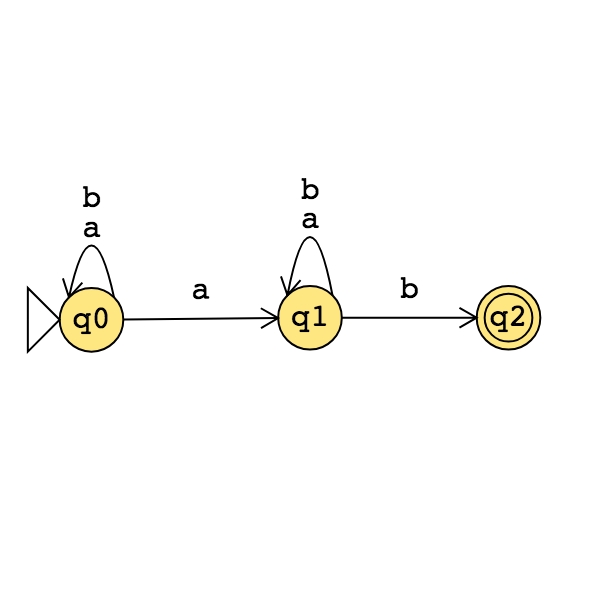
\includegraphics[width=2.5in]{../../resources/machines/Lect6NFA1.png}


The language recognized by this NFA is



The state diagram of a DFA recognizing this same language is:

\vspace{70pt}
Suppose $A$ is a language over an alphabet $\Sigma$.
{\bf Claim:} if there is a NFA $N$ such that $L(N) = A$ then 
there is a DFA $M$ such that $L(M) = A$.

{\bf Proof idea}: States in $M$ are ``macro-states" -- collections of states from $N$ -- 
that represent the set of possible states a computation of $N$ might be in.


{\bf Formal construction}: Let $N = (Q, \Sigma, \delta, q_0, F)$.  Define 
\[
M = (~ \mathcal{P}(Q), \Sigma, \delta', q',  \{ X \subseteq Q \mid X \cap F \neq \emptyset \}~ )
\]
where $q' = \{ q \in Q \mid \text{$q = q_0$ or is accessible from $q_0$ by spontaneous moves in $N$} \}$
and 
\[
    \delta' (~(X, x)~) = \{ q \in Q \mid q \in \delta( ~(r,x)~) ~\text{for some $r \in X$ or is accessible 
from such an $r$ by spontaneous moves in $N$} \}
\]

\vfill

\newpage
Consider the state diagram of an NFA over $\{0,1\}$. Use the ``macro-state'' construction 
to find an equivalent DFA.


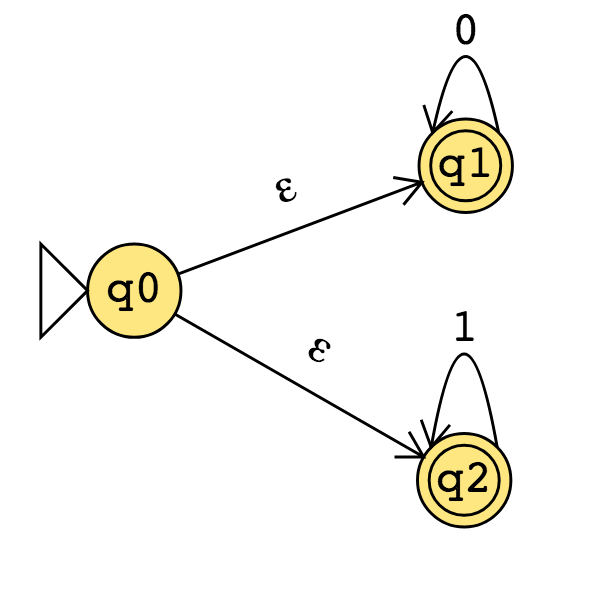
\includegraphics[width=1.8in]{../../resources/machines/Lect6NFA2.png}

\vspace{50pt}

Prune this diagram to get an 
equivalent DFA 
with only the ``macro-states" reachable from the start state.

\vspace{150pt}

Suppose $A$ is a language over an alphabet $\Sigma$.
{\bf Claim:} if there is a regular expression $R$ such that $L(R) = A$, then there is a NFA, let's call it $N$, such that 
$L(N) = A$.

{\bf Structural induction}: Regular expression is built from basis regular expressions using inductive steps
(union, concatenation, Kleene star symbols). Use constructions to mirror these in NFAs.


{\bf Application}: A state diagram for a NFA over $\{a,b\}$ that recognizes $L(a^* (ab)^*)$:

\vfill

\newpage

Suppose $A$ is a language over an alphabet $\Sigma$.
{\bf Claim:} if there is a DFA $M$ such that $L(M) = A$, then there is a regular expression, let's call it $R$, such that 
$L(R) = A$.

{\bf Proof idea}: Trace all possible paths from start state to accept state.  Express labels of these paths
as regular expressions, and union them all.

\begin{enumerate}
\item Add new start state with $\varepsilon$ arrow to old start state.
\item Add new accept state with $\varepsilon$ arrow from old accept states.  Make old accept states
non-accept.
\item Remove one (of the old) states at a time: modify regular expressions on arrows that went through removed
state to restore language recognized by machine.
\end{enumerate}

{\bf Application}: Find a regular expression describing the language recognized by the DFA with 
state diagram

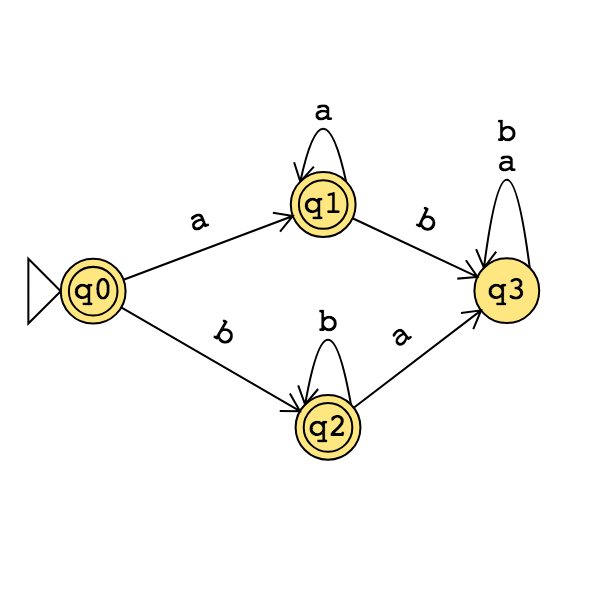
\includegraphics[width=2.5in]{../../resources/machines/Lect6NFA3.png}

\vfill


\newpage

{\bf Conclusion}: For each language $L$,
\begin{center}
    {\bf There is a DFA that recognizes $L$ \qquad $\exists M ~(M \textrm{ is a DFA and } L(M) = A)$}\\
    {\bf if and only if}\\
    {\bf There is a NFA that recognizes $L$  \qquad $\exists N ~(N \textrm{ is a NFA and } L(N) = A)$}\\
    {\bf if and only if}\\
    {\bf There is a regular expression that describes $L$ $\exists R ~(R \textrm{ is a regular expression and } L(R) = A)$}\\
\end{center}

A language is called {\bf regular} when any (hence all) of the above three conditions are met. \vfill
\section*{Week2 friday}



\begin{center}
\begin{tabular}{|ll|}
\hline
\multicolumn{2}{|l|}{{\bf Nondeterministic finite automaton} $M = (Q, \Sigma, \delta, q_0, F)$} \\
Finite set of states $Q$  & Can  be labelled by any collection  of distinct names. Default: $q0, q1, \ldots$  \\
Alphabet $\Sigma$ &  Each input to the automaton is a string over  $\Sigma$. \\
Arrow labels $\Sigma_\varepsilon$ &  $\Sigma_\varepsilon = \Sigma \cup \{ \varepsilon\}$. \\
&  Arrows 
in the state diagram are labelled either by symbols from $\Sigma$ or by $\varepsilon$ \\
Transition function $\delta$  & $\delta: Q \times \Sigma_{\varepsilon} \to \mathcal{P}(Q)$
gives the {\bf set of possible next states} for a transition \\
&  from the current state upon reading a symbol or spontaneously moving.\\
Start state $q_0$ & Element of $Q$.  Each computation of the machine starts at the  start  state.\\
Accept (final) states $F$ & $F \subseteq  Q$.\\
$M$ accepts the input string & if and only if {\bf there is} a computation of $M$ on the input string\\
&  that 
processes the whole string and ends in an
accept state.\\
\hline
{\it Page 53}& \\
\hline
\end{tabular}
\end{center}

The formal definition of the NFA over $\{0,1\}$ given by this state diagram is: 

\includegraphics[width=2in]{../../resources/machines/Lect4NFA1.png}

The language over $\{0,1\}$ recognized by this NFA is:

\vspace{70pt}

Change the transition function to get a different NFA which accepts
the empty string.


\newpage

The state diagram of an NFA over $\{a,b\}$ is below.  The formal definition of this NFA is:

\vspace{-30pt}

\includegraphics[width=2.5in]{../../resources/machines/Lect5NFA1.png}


\vspace{-10pt}

The language recognized by this NFA is:  \vfill
\end{document}